%!TEX root = Manuscrit.tex
\chapter{Jeux de données en télédétection}

%\subsection{Jeux de données en télédétection}

Il existe plusieurs jeux de données pour la classification d'images optiques de télédétection. Citons ainsi les jeux de données UC Merced~\cite{yang_bag--visual-words_2010} contenant 2 100 images aériennes dans 21 classes d'occupation des sols, Brazilian Coffe~\cite{penatti_deep_2015} d'images \gls{SPOT} pour la classification de terrains cultivés et SAT-4/SAT-6~\cite{basu_deepsat_2015} contenant respectivement 500 000 et 405 000 images aériennes pour plusieurs classes d'occupation des sols. L'inconvénient de ces jeux de données est d'une part la faible taille des images (256$\times$\SI{256}{\px} pour UC Merced et Brazilian Coffe, 28$\times$\SI{28}{\px} pour SAT) et la faible quantité d'annotations. En effet, ces jeux de données, prévus pour la classification, ne peuvent que difficilement être utilisés pour la segmentation sémantique. Cependant, plusieurs jeux de données comprenant des annotations denses ont été proposés.

\section{ISPRS 2D Semantic Labeling}

\begin{figure}[t]
		\foreach\picid in {7,21,28}{%
		\begin{subfigure}{0.33\textwidth}
			\includegraphics[angle=90,width=\textwidth]{vaihingen_top_\picid}
			\caption*{Image RVB}
		\end{subfigure}%
		\begin{subfigure}{0.33\textwidth}
			\includegraphics[angle=90,width=\textwidth]{vaihingen_ndsm_\picid}
			\caption*{\gls{MNH}}
		\end{subfigure}%
		\begin{subfigure}{0.33\textwidth}
			\includegraphics[angle=90,width=\textwidth]{vaihingen_gt_\picid}
			\caption*{Vérité terrain}
		\end{subfigure}
		}
    \caption{Images ortho-rectifiées et \gls{MNH} pour le jeu de données ISPRS Vaihingen .}
    \label{fig:isprs_vaihingen}
\end{figure}

\begin{figure}[t]
		\foreach\picid in {3_10,6_11}{%7_12}{%
		\begin{subfigure}{0.33\textwidth}
			\includegraphics[width=\textwidth]{potsdam_top_\picid}
			\caption*{Image RVB}
		\end{subfigure}%
		\begin{subfigure}{0.33\textwidth}
			\includegraphics[width=\textwidth]{potsdam_ndsm_\picid}
			\caption*{\gls{MNH}}
		\end{subfigure}%
		\begin{subfigure}{0.33\textwidth}
			\includegraphics[width=\textwidth]{potsdam_gt_\picid}
			\caption*{Vérité terrain}
		\end{subfigure}
		}
	\caption{Images ortho-rectifiées et \gls{MNH} pour le jeu de données ISPRS Potsdam.}
	\label{fig:isprs_potsdam}
\end{figure}

Le jeu de données ISPRS 2D Semantic Labeling~\cite{rottensteiner_isprs_2012} est constitué de deux ensembles d'images aériennes \glsfirst{THR}. Dans les deux cas, il s'agit de scènes urbaines disposant de cinq classes d'intérêt pour la segmentation sémantique\,: surfaces imperméables (routes, parkings, trottoirs\dots), bâtiments, végétation basse, arbres et véhicules. Une classe de rejet est également définie et comprend le mobilier urbain (bancs, poubelles, conteneurs\dots) et les surfaces inclassables (terrains de basketball, zones en travaux, points d'eau\dots).

Le jeu de données se décline en deux scènes. La première est issue d'une acquisition aéroportée sur la ville de Vaihingen (Allemagne) et comporte une mosaïque de 33 tuiles \gls{IRRV} ortho-rectifiées à une résolution de \SI{9}{\centi\meter/\px}. L'acquisition optique est accompagnée d'une acquisition \gls{Lidar} à la même résolution, dont a été extrait un \gls{MNE}. Un \gls{MNH} pré-calculé~\cite{gerke_use_2015} dérivé du \gls{MNE} est également disponible. Les ortho-images sont fournies en format \gls{TIFF} encodés sur 8 bits, tandis que le \gls{MNE} est fourni en flottant sur 32 bits. Toutes les données ont été recalées sur la même grille de pixels. Les images ont une taille moyenne d'environ $2600\times1900$px, soit une surface d'approximativement $40 000m^2$. Vaihingen est une ville de taille moyenne (28 853 habitants en 2009), caractérisée par une urbanisation moyenne composée majoritairement de pavillons résidentiels et d'espace verts urbains.

La seconde scène est une acquisition aéroportée sur la ville de Potsdam (Allemagne) et comporte une mosaïque de 38 tuiles \gls{IRRVB} à une résolution de \SI{5}{\centi\meter/\px}. Les tuiles présentent toutes les mêmes dimensions, à savoir $6000\times6000$px, soit une surface de \SI{90 000}{\meter\squared}. Un \gls{MNE} et un \gls{MNH} dérivé sont également fournis. Des annotations denses sont disponibles pour les mêmes classes que précédemment sur 24 images. À nouveau, l'ensemble des modalités sont recalées sur la même grille de pixels et les images sont fournies en \gls{TIFF} sur 8 bits, tandis que les modèles de surface sont fournis en flottant sur 32 bits. Potsdam est une ville urbanisée relativement grande (161 468 habitants en 2013), caractérisée par de nombreux immeubles, un réseau routier dense. À noter la présence d'un canal et de nombreux travaux de construction à la date de l'acquisition des images.

Quelques exemples représentatifs des deux acquisitions sont montrés dans les~\cref{fig:isprs_vaihingen,fig:isprs_potsdam}.

Les images dont les annotations ne sont pas rendues publiques servent à évaluer en aveugle les méthodes proposées par la communauté. La commission WG II/4 de l'\gls{ISPRS} gère ainsi un tableau de résultat public\footnote{\url{http://www2.isprs.org/commissions/comm2/wg4/vaihingen-2d-semantic-labeling-contest.html}}\footnote{\url{http://www2.isprs.org/commissions/comm2/wg4/potsdam-2d-semantic-labeling.html}}, détaillant les performances obtenues par différentes méthodes de l'état-de-l'art.

\section{Data Fusion Contest 2015}

\begin{figure}[t]
		\foreach\picid in {1,2}{%
		\begin{subfigure}{0.33\textwidth}
			\includegraphics[width=\textwidth]{dfc2015_top\picid}
			\caption*{Image RVB}
		\end{subfigure}%
		\begin{subfigure}{0.33\textwidth}
			\includegraphics[width=\textwidth]{dfc2015_dsm\picid}
			\caption*{\gls{MNH}}
		\end{subfigure}%
		\begin{subfigure}{0.33\textwidth}
			\includegraphics[width=\textwidth]{dfc2015_gt\picid}
			\caption*{Vérité terrain}
		\end{subfigure}
		}
	\caption{Images ortho-rectifiées et \gls{MNH} pour le jeu de données \gls{DFC} 2015.}
	\label{fig:dfc2015}
\end{figure}

Le jeu de données \gls{DFC} 2015~\cite{campos-taberner_processing_2016} est issu d'une compétition de fusion de données organisée par le groupe de travail \gls{GRSS} de l'\gls{IEEE}. Ce jeu de données comporte une mosaïque de 7 images couleurs ortho-rectifiées de dimensions $10 000\times10 000$ à une résolution au sol de \SI{5}{\centi\meter/\px}, soit une surface par tuile de \SI{250 000}{\meter\squared}. L'acquisition a été réalisée sur la zone portuaire de Zeebruges (Belgique) en mars 2011. Il est accompagné d'une acquisition \gls{Lidar} comprenant environ \SI{65}{points/\meter\squared} espacés chacun de \SI{10}{\centi\meter}. Les données couleurs sont fournies en \gls{TIFF} encodé sur 8 bits et les données \gls{Lidar} sont fournis rastérisées sous la forme d'un \gls{MNE} en flottant sur 32 bits, ainsi qu'un nuage de points. Des annotations denses réalisées par l'\gls{ONERA} sont disponibles pour les classes bateau, voiture, végétation basse, arbre, bâtiment, eau et surface imperméable. La~\cref{fig:dfc2015} montre quelques exemples d'images extraites du jeu de données.

Un tableau de résultats public est maintenu par l'\gls{IEEE} \gls{GRSS}\footnote{\url{http://dase.ticinumaerospace.com/}}.

\section{Data Fusion Contest 2017}

Le jeu de données \gls{DFC} 2017~\cite{tuia_2017_2017} contient une variété d'images satellites issues de Landsat et Sentinel-2, rééchantillonnées à une résolution spatiale de \SI{100}{\meter/\px} ainsi que des tuiles OpenStreetMap rastérisées à \SI{20}{\meter/\px} contenant les empreintes de bâtiments et les annotations des utilisateurs pour les classes d'occupations du sol. Des annotations partielles sont fournies contenant les 17 zones climatiques locales définies par~\citet{stewart_local_2012}.

Un tableau de résultats public est maintenu par l'\gls{IEEE} \gls{GRSS}\footnote{\url{http://dase.ticinumaerospace.com/}}.

\section{Data Fusion Contest 2018}

\begin{figure}[t]
  \begin{subfigure}{\textwidth}
    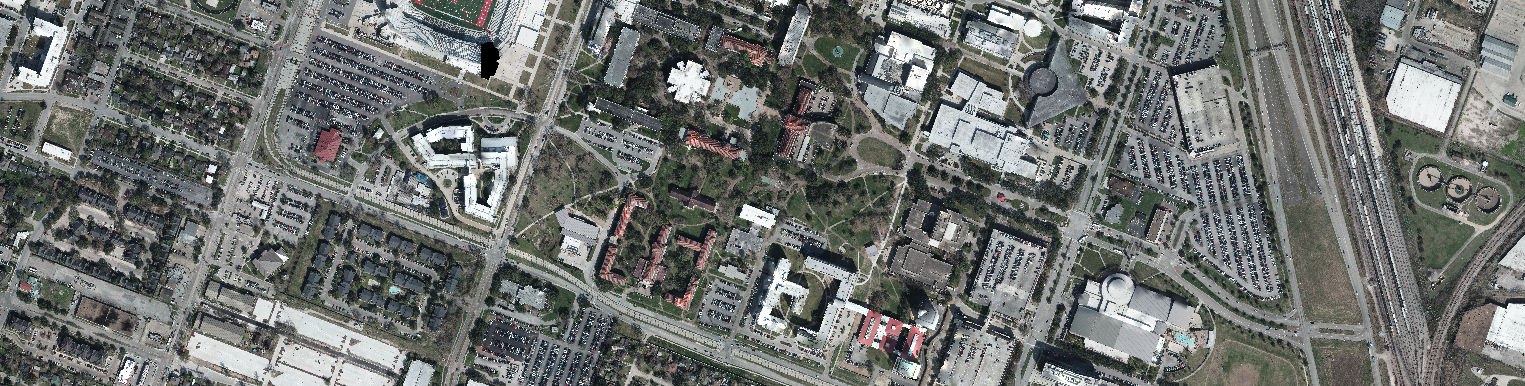
\includegraphics[width=\textwidth]{dfc2018_top}
    \caption{Image \gls{RVB}}
  \end{subfigure}
  \begin{subfigure}{\textwidth}
    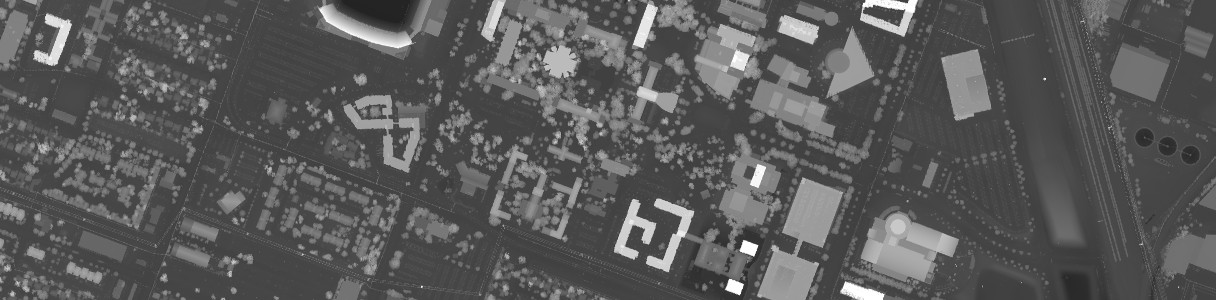
\includegraphics[width=\textwidth]{dfc2018_dsm}
    \caption{\gls{MNH}}
  \end{subfigure}
  \begin{subfigure}{\textwidth}
    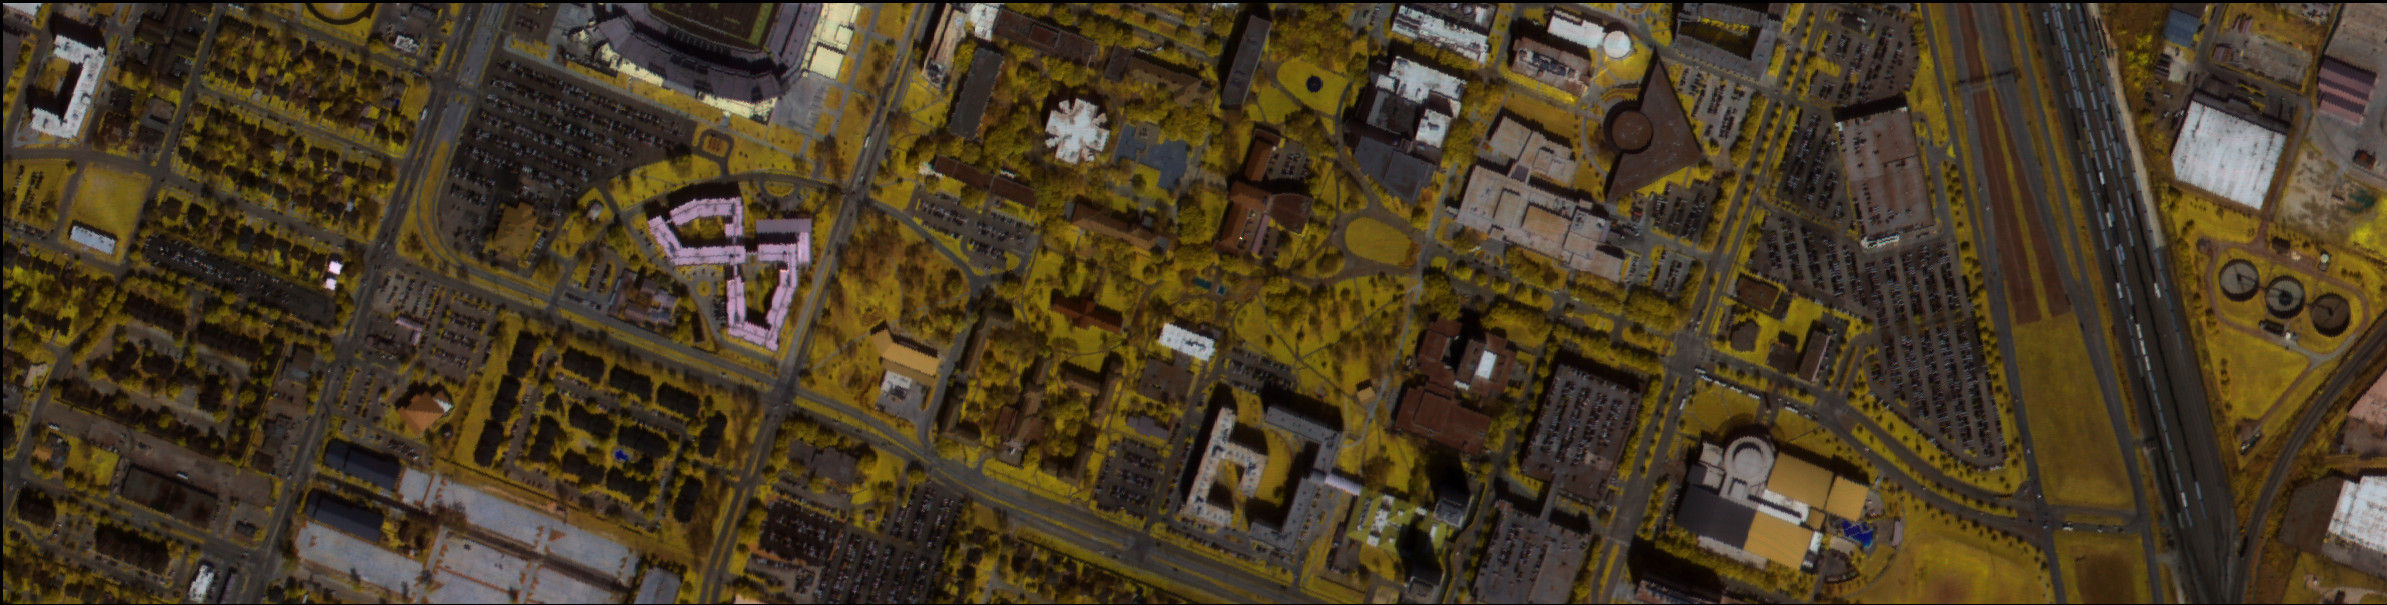
\includegraphics[width=\textwidth]{dfc2018_hsi}
    \caption{Image hyperspectrale (fausses couleurs)}
  \end{subfigure}
  \begin{subfigure}{\textwidth}
    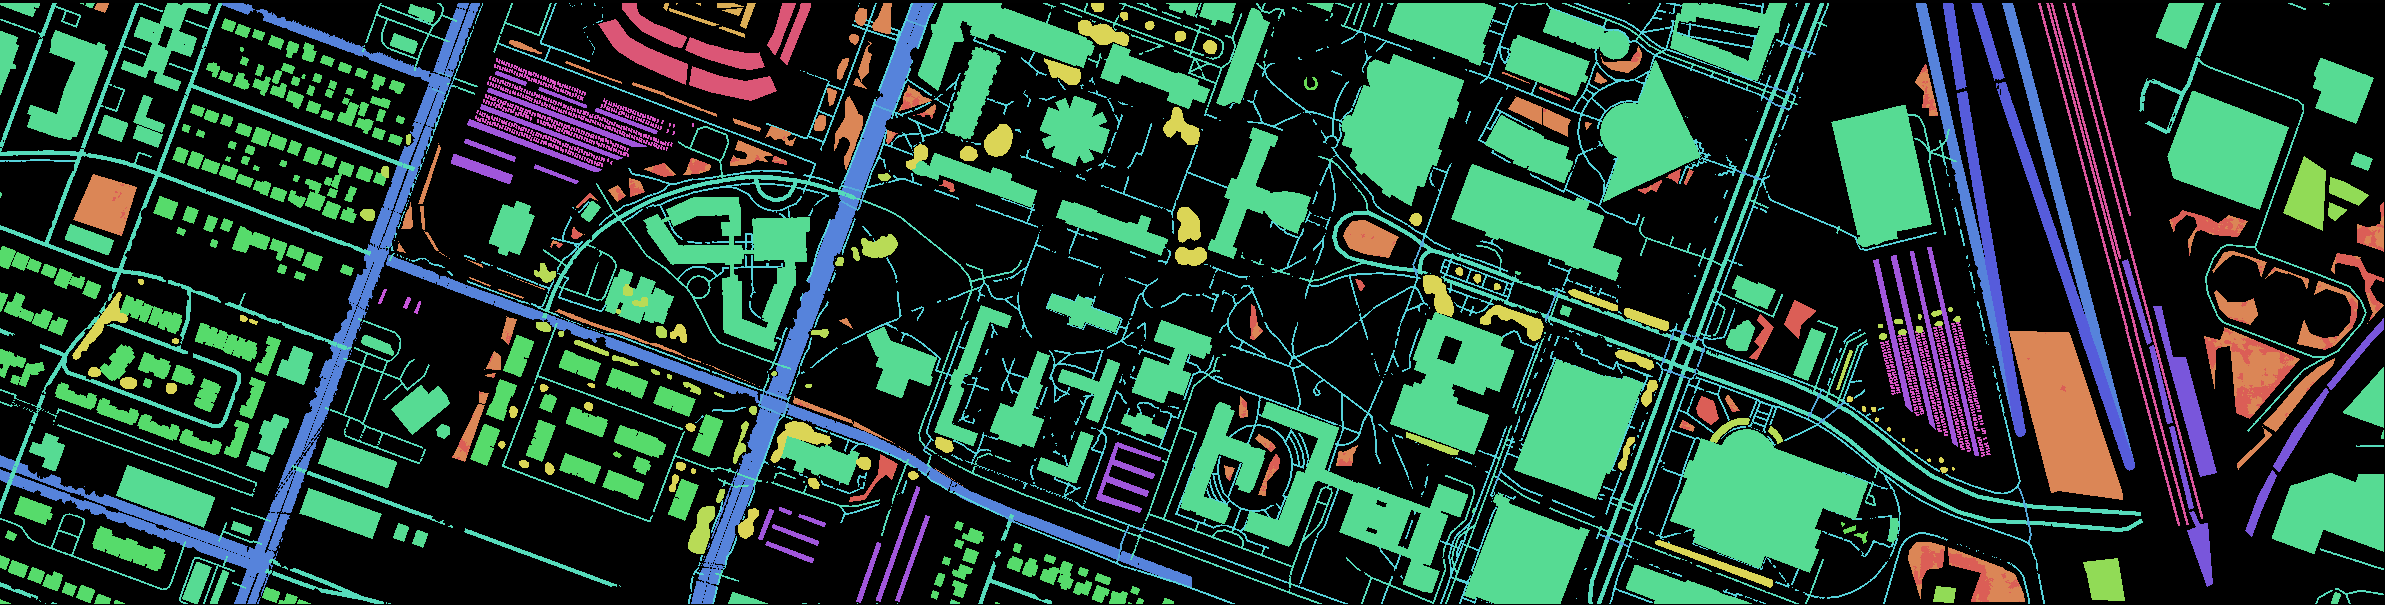
\includegraphics[width=\textwidth]{dfc2018_gt}
    \caption{Vérité terrain}
  \end{subfigure}
  \caption{Données d'entraînement du concours \gls{DFC} 2018.}
  \label{fig:dfc2018}
\end{figure}

Le jeu de données \gls{DFC} 2018~\cite{le_saux_2018_2018} contient 14 images aériennes \gls{RVB} ortho-rectifiées \gls{THR} à \SI{5}{\centi\meter/\px} de dimensions $12000\times12000$, accompagnées par une image hyperspectrale à 48 bandes à \SI{1}{\meter/\px}. Une acquisition \gls{Lidar} multispectrale est également disponible à une résolution de \SI{0,5}{\meter/\px}, dont est dérivé un \gls{MNH}. Des annotations partielles sont fournies pour la moitié du jeu de données sur diverses classes d'intérêt urbaines, l'autre moitié des annotations étant conservées secrètes pour l'évaluation. Le jeu d'apprentissage est illustré par la~\cref{fig:dfc2018}.

Un tableau de résultats public est maintenu par l'\gls{IEEE} \gls{GRSS}\footnote{\url{http://dase.ticinumaerospace.com/}}.

\section{Inria Aerial Image Labeling}

\begin{figure}[t]
  \foreach \picpath\picname in {chicago5_top/Ortho-image (Chicago),chicago5_gt/Vérité terrain (Chicago),vienna2_top/Ortho-image (Vienne),vienna2_gt/Vérité terrain (Vienne)}{%
  \begin{subfigure}[t]{0.25\textwidth}%
    \includegraphics[width=\textwidth]{\picpath}%
    \caption*{\picname}
  \end{subfigure}%
  }
  \caption{Exemples d'images extraites de la base de données \emph{Inria Aerial Image Labeling}.}
  \label{fig:inria}
\end{figure}

Le jeu de données \emph{Inria Aerial Image Labeling}~\cite{maggiori_can_2017} contient 360 images \gls{RVB} ortho-rectifiées de taille $5000\times5000$px à une résolution de 30cm/px, soit une surface de $2,25km²$. Les images ont été compilées depuis plusieurs sources gouvernementales à des résolutions diverses. Il s'agit néanmoins systématiquement d'acquisitions aéroportées, ortho-rectifiées et ré-échantillonnée à 30cm/px si besoin. Les acquisitions ont été réalisées sur 10 agglomérations de divers points du globe. La moitié des villes sont utilisées pour associées à des annotations publiques d'empreintes de bâtiments provenant de sources cadastrales. Ces images peuvent être utilisées pour l'entraînement de modèles d'extraction de bâtiments. Le reste du jeu de données est réservé à l'évaluation des modèles. Quelques images et annotations du jeu d'apprentissage sont illustrées dans la~\cref{fig:inria}.

Les organisateurs gèrent un tableau de résultats public\footnote{\url{https://project.inria.fr/aerialimagelabeling/leaderboard/}} permettant de comparer les performances obtenues par différentes méthodes.
